\documentclass[apjl]{emulateapj}

\shorttitle{shorttitle}
\shortauthors{shortauthors}


%%% packages
\usepackage{graphicx}
\usepackage{amsmath}
\usepackage{xspace}
%\usepackage{array}
\usepackage{lineno}

\newcommand{\myemail}{email@email.com}

\begin{document}
\linenumbers

\title{Spin-orbit misalignment for the long period companion of KOI-368}

\author{First Author\altaffilmark{1} and
Second Author\altaffilmark{2}}

\altaffiltext{1}{Affil2; \email{\myemail}}
\altaffiltext{2}{Affil1}

\begin{abstract}
Abstract
\end{abstract}

\keywords{keywords}

\section{Introduction}
\label{sec:introduction}

\section{Method}
\label{sec:method}

\subsection{Host star parameters}
\label{sec:host-star-parameters}

[APO observation and spectrum fitting]

We estimate the rotation period of the host star by plotting the
Lomb-Scargle periodogram
\citep[][Figure~\ref{fig:LS}]{1976Ap&amp;SS..39..447L,1982ApJ...263..835S}
for the Kepler PDC long cadence lightcurve, with primary transits masked. The
resulting peaks was checked by the CLEAN algorithm
\citep{1987AJ.....93..968R}. We adopte the first significant peak at 1.19 days as
the rotation period of the host star. [Justify with vsini]

\begin{figure}[h!]
  \centering
  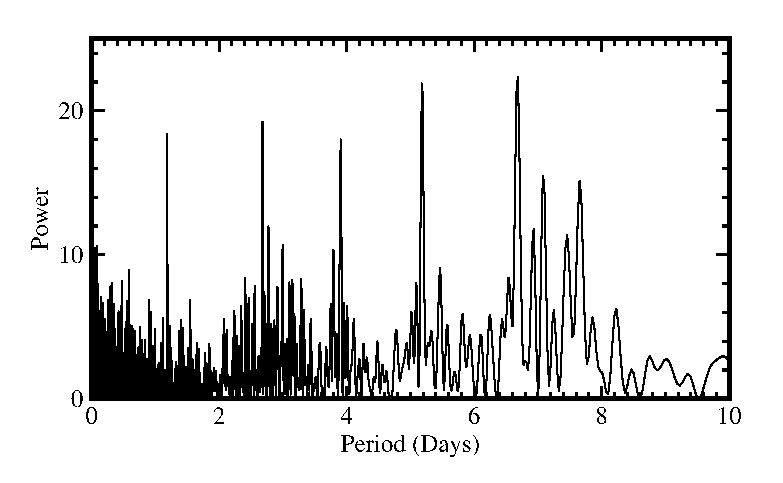
\includegraphics[width=7cm]{LS.eps}
  \caption{Lomb-Scargle periodogram of the PDC lightcurve, with the
    transits masked out. The lightcurve is rotationally modulated with
  a period of 1.19 days.}
  \label{fig:LS}
\end{figure}

\subsection{Transit lightcurve fitting}
\label{sec:transit-light-curve}

The transit lightcurve is modelled using the
\citet{1972ApJ...174..617N} model, implemented in an adaption of the
JKTEBOP code \citep{1981AJ.....86..102P,2004MNRAS.351.1277S}. The
relevant free parameters are orbital period $P$, transit centre $T_0$,
normalised radius sum $R_\star+R_p / a$, radius ratio $R_p/R_\star$,
line of sight inclination $i$, and quadratic limb darkening
coefficients $c_1$ and $c_2$. Initial estimates of the limb darkening
coefficients are taken from \citet{2010A&amp;A...510A..21S}. Jump
parameters for the stellar oblation correction include the planet
orbit obliquity $\lambda$, stellar oblation $f$. The projection angle
between the stellar rotation axis and line of sight $i_\text{rot}$ is
fixed for the initial analysis, then set free to explore the potential
degeneracies. A flux offset for each transit event is calculated and
removed at each iteration, and is not included in the fit
parameters. For Kepler long cadence data, the model is modified by a
30 minute boxcar smooth. The best fit parameters and the posterior
probability distribution is explored via a Markov chain Monte Carlo
(MCMC) analysis, using the \emph{emcee} MCMC ensemble sampler
\citep{2012arXiv1202.3665F}. The likelihood function is given by
$\exp(-\Delta\chi^2/2)$. For each transit, we scale the flux errors such
that the reduced $\chi^2$ is at unity. This allows for errors other
than photon noise to be taken into account.

% Figure X plots 



\section{Analysis}
\label{sec:analysis}

\section{Discussion}
\label{sec:discussion}

\bibliographystyle{apj}
\bibliography{mybibfile}

\end{document}
